\section{Inngangur}
Verkefnið sem við ætlum að gera (Kjartan og Einar) er að búa til miðunartæki á milli 2 tækja með notkun GPS. Þetta getur verið notað til þess að miða t.d sensora, loftnetum, laserum o.sf frá einum object yfir á annan frá löngum vegalendum. Það verða tveir hlutir sem þarf að búa til, Base og Target (Það gæti samt verið hægt að nota síman sem target og við munum líta betur á það). Eina sem Target-ið á að gera er að fá GPS staðsetninguna á sjálfum sér, þátta gögnin frá því og senda það til baka á Base. Base mun þá fá upplýsingarnar um GPS-Staðsetninguna hjá Target og reiknar svo út frá sýnar eigin GPS Staðsetningu til að fá það sem kallast Positive Vector. Við munum nota forritið Arduino IDE fyrir kóðann sem þarf að innihalda eftirfarandi libraries : Software Serial, TinyGPS og Servo. Þetta verkefni hefur marga tilganga nú þegar í heiminum, eins og GPS í símum ef þú ert að reyna finna út hvernig þú kemst til Fjörðin í Hafnafirði, þá reiknar það út frá staðsetninguni þinni til staðsetninguna sem þú vilt fara og finnur út leiðina til að komast þangað fyrir þig, og það er líka notað til að finna og fylgjast með flugtæki og miðla. GPS er rosa frábær uppfinning sem gefur manni tækifæri til að gera eitthvað skemmtilegt og notfærilegt í nútíma-tækni heimi sem tekur til staðar í dag. Gervitunglið sem er notað í GPS-inn gerir mest af vinnunni þannig að GPS-recieverinn getur verið mjög lítill og einfaldur. Nú þegar GPSinn er svo vinsæll í dag og heldur áfram að verða nákvæmnari og nákvæmnari, hafa forrit á mörgum sviðum verið sprengd upp. Sum af þessum innifela sjálfstjórnandi bíla, aðstoðar lendingum flugvéla og margt fleira. GPS-reciever er breytilegur í kostnaði eftir nákvæmni, þannig að rétti reciever þarf að vera valin fyrir viðkomandi umsókn. Svo nýtist þetta fyrir þá sem vilja búa til GPS-tengingu fyrir þeirra eigin notkun eins og fyrir eitthvað forrit eða verkefni eða bara fyrir sitt eigið áhugamál, og fyrir mjög lítinn pening! Oftast þegar þú kaupir svona GPS-reciever þá kostar það mun meira heldur en að búa bara til það sjálfur. Og ef það er eitthvað sem þú vilt fornast að týna í framtíðinni, þá geturu bara sett GPS-reciever á það og þá muntu fara létt með það að finna það aftur :). Svo margt getur verið hægt með notkun GPS, það getur hjálpað fólk með sú einföldustu verkefni, alveg til sú erfiðustu, og líka notað fyrir venjulega dags daglega hluti, eins og að þurfa finna leið útí Dominos í Skeifunni, eða búa til litla sjálfvirka teygjubyssu sem getur miðað sjálf á eitthvað Target, eða notað þetta til að halda upplýsingar á staðsetningu flugvéla, sem getur hjálpað að stýra þá burt frá slæmum aðstæðum í loftinu. Þetta verður frábært tækifæri til þess að geta notað GPSinn fyrir sjálfan sig og prufa að búa til mjög einfaldan en sniðugan robot sem getur fundið hvar sem GPS-recieverinn er, nærrum alveg sjálfkrafa.
\begin{figure}[h]
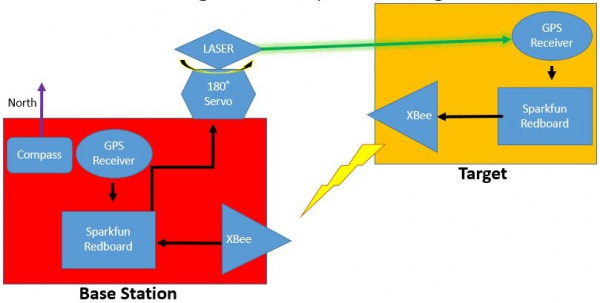
\includegraphics[scale=.3]{img/system}
\end{figure}
